\documentclass[12pt,a4paper]{article}
\usepackage[utf8]{inputenc}
\usepackage[spanish]{babel}
\usepackage{mathptmx} % Fuente Times New Roman (APA 7)
\usepackage{graphicx}
\usepackage{geometry}
% Márgenes APA: 1 pulgada (2.54 cm) en todos los lados
\geometry{top=2.54cm, bottom=2.54cm, left=2.54cm, right=2.54cm}
\usepackage{float}
\usepackage{hyperref}
\usepackage{url}
\usepackage{booktabs} % Para tablas formato APA 7
\usepackage{amsmath}  % Para ecuaciones y fórmulas matemáticas

% ---------------------------------------------------------
% CONFIGURACIONES ESTRICTAS APA 7ma EDICIÓN
% ---------------------------------------------------------
\usepackage{setspace}
\doublespacing

\usepackage{indentfirst}
\setlength{\parindent}{1.27cm}

\usepackage{caption}
\captionsetup[figure]{
    name=Figura,
    labelsep=newline,
    justification=raggedright,
    singlelinecheck=false,
    labelfont=bf,
    textfont=it
}
\captionsetup[table]{
    labelsep=newline,
    justification=raggedright,
    singlelinecheck=false,
    labelfont=bf,
    textfont=it
}

\usepackage{titlesec}
% Nivel 1: Centrado, Negrita, Tamaño 12pt
\titleformat{\section}[block]{\normalfont\normalsize\bfseries\centering}{}{0em}{}
% Nivel 2: Izquierda, Negrita, Tamaño 12pt
\titleformat{\subsection}[block]{\normalfont\normalsize\bfseries}{}{0em}{}


\begin{document}

% ---------------------------------------------------------
% PORTADA
% ---------------------------------------------------------
\begin{titlepage}
    \singlespacing
    \setlength{\parindent}{0cm}
    \centering
    {\bfseries\Large UNIVERSIDAD NACIONAL DEL ALTIPLANO \par}
    \vspace{0.4cm}
    {\bfseries\large FACULTAD DE INGENIERÍA DE MECÁNICA ELÉCTRICA, INGENIERÍA ELECTRÓNICA E INGENIERÍA DE SISTEMAS \par}
    \vspace{0.4cm}
    {\bfseries\large ESCUELA PROFESIONAL DE INGENIERÍA DE SISTEMAS \par}
    
    \vspace{0.8cm}
    
\includegraphics[width=0.35\textwidth]{imagenes/logo.png}\par
    \vspace{0.8cm}
    
    {\bfseries\Large Interfaz de la gestión de disco \par}
    
    \vspace{1.2cm}
    
    {\bfseries CURSO.} \par
    SISTEMAS OPERATIVOS \par
    
    \vspace{0.5cm}
    {\bfseries DOCENTE.} \par
    RUELAS ACERO DONIA ALIZANDRA \par
    
    \vspace{0.5cm}
    {\bfseries ALUMNO.} \par
    ABAD POMA MAQUERA \par
    
    \vspace{0.5cm}
    {\bfseries CODIGO.} \par
    241177 \par
    
    \vspace{0.5cm}
    {\bfseries QUINTO SEMESTRE} \par
    {\bfseries 2026 – I} \par
    
    \vfill
    {\bfseries PUNO – PERÚ} \par
\end{titlepage}

\newpage
\doublespacing
\setlength{\parindent}{1.27cm}

% ---------------------------------------------------------
% 1. INTRODUCCIÓN
% ---------------------------------------------------------
\section{Introducción}

Uno de los temas que más se discuten en la teoría de Sistemas Operativos, pero que pocas veces se logra visualizar de forma práctica, es la manera en que el sistema operativo decide dónde guardar cada archivo dentro del disco. Cuando se guarda un documento, el sistema tiene que responder de inmediato: ¿guardo los bloques juntos o los reparto por donde haya espacio? Esa decisión, que parece simple, tiene un impacto enorme en el rendimiento del sistema a largo plazo, ya que afecta tanto la velocidad de lectura como el aprovechamiento real del espacio disponible.

Este informe documenta el desarrollo de SimuKernel, un simulador interactivo desarrollado por el autor para poder visualizar de primera mano cómo funcionan los tres métodos más importantes de asignación de espacio en disco: Contigua, Enlazada e Indexada. En lugar de quedarse únicamente con la teoría del libro, el objetivo fue construir una herramienta que permitiera comparar en tiempo real qué pasa con el disco cuando se usa cada método, cuántas operaciones genera y qué tan fragmentado queda el almacenamiento.

% ---------------------------------------------------------
% 2. OBJETIVO GENERAL
% ---------------------------------------------------------
\section{Objetivo General}

Desarrollar y documentar una interfaz gráfica interactiva orientada a simular, de forma visual y paso a paso, el comportamiento algorítmico de los métodos de asignación de espacio en disco (Contigua con variantes First Fit y Best Fit, Enlazada e Indexada), permitiendo la evaluación técnica del rendimiento de Entrada/Salida, el análisis de fragmentación y la comprensión del directorio de metadatos del sistema de archivos, todo ello mediante métricas calculadas en tiempo real.

% ---------------------------------------------------------
% 3. MARCO TEÓRICO
% ---------------------------------------------------------
\section{Marco Teórico}

Para construir el simulador con rigor, el trabajo partió de los tres modelos de asignación que aparecen en la bibliografía clásica de Sistemas Operativos. A continuación se explica cómo funciona cada uno y qué implicaciones tiene su uso en la práctica.

\subsection{Asignación Contigua}

Este método exige que el archivo se almacene en una secuencia ininterrumpida de bloques físicos dentro del disco. Su principal ventaja radica en el altísimo rendimiento durante la lectura secuencial; al estar los bloques adyacentes, el cabezal del disco realiza una única operación de búsqueda y lee la información de forma continua. Sin embargo, este enfoque adolece gravemente de un fenómeno conocido como fragmentación externa. A medida que se crean y eliminan archivos de diferentes tamaños, el disco comienza a llenarse de pequeños huecos libres dispersos. Con el tiempo, aunque la suma total de estos huecos sea suficiente para almacenar un archivo nuevo, el sistema operativo denegará la operación porque no existe un único hueco continuo del tamaño requerido.

El usuario define la entrada con tres campos por archivo: nombre, bloque de inicio y longitud en bloques. Para gestionar automáticamente la búsqueda del espacio libre, el simulador incorpora dos estrategias adicionales: el método \textit{First Fit} (Primer Ajuste), que recorre el mapa del disco desde el bloque cero y asigna el primer hueco libre que tenga capacidad suficiente, logrando una asignación muy rápida; y el método \textit{Best Fit} (Mejor Ajuste), que escanea la totalidad del disco buscando el hueco libre que más se ajuste al tamaño del archivo, minimizando el espacio sobrante, aunque a costa de un mayor tiempo de procesamiento.

\subsection{Asignación Enlazada}

A diferencia de la asignación contigua, el método enlazado elimina la restricción de adyacencia. El archivo puede estar disperso y fragmentado en cualquier bloque libre del disco. Para mantener la cohesión del archivo, cada bloque de datos almacena, además de la información del usuario, un pequeño puntero (configurable en el simulador, con un valor predeterminado de 4 bytes) que indica la dirección lógica del siguiente bloque de la secuencia. El último bloque de la cadena lleva un puntero especial con valor \texttt{-1}, indicando el fin del archivo. De esta forma, el directorio del sistema solo necesita conocer el bloque de inicio y el bloque final.

Si bien esta solución erradica por completo la fragmentación externa, introduce dos problemas significativos. El primero es la sobrecarga de espacio, ya que un porcentaje de cada bloque se sacrifica para guardar el puntero; el simulador calcula automáticamente los ``datos útiles por bloque'' como \texttt{tamaño\_bloque -- tamaño\_puntero}. El segundo es la ineficiencia en el acceso directo: si se necesita leer el bloque cincuenta de un archivo, el sistema operativo está obligado a leer secuencialmente los cuarenta y nueve bloques anteriores para seguir el rastro de punteros.

\subsection{Asignación Indexada}

La asignación indexada nace como una solución híbrida para resolver el problema del acceso aleatorio de las listas enlazadas, sin caer en la fragmentación externa de la asignación contigua. Este método dedica un bloque de disco entero, conocido como bloque índice, exclusivamente a almacenar las direcciones de todos los bloques de datos del archivo. La capacidad máxima de este bloque índice está determinada por la fórmula: \texttt{máx\_índices = tamaño\_bloque / tamaño\_puntero}. Para un bloque de 512 bytes y un puntero de 4 bytes, el bloque índice puede referenciar hasta 128 bloques de datos.

Cuando se crea un archivo, el bloque índice se escribe primero y en él se anotan todas las direcciones. Si el sistema necesita el bloque de datos número cincuenta, simplemente lee el índice y salta directamente a la ubicación física, sin lecturas intermedias. Sin embargo, el simulador evidencia la principal desventaja: el espacio desperdiciado en el bloque índice se calcula como \texttt{tamaño\_bloque -- (cantidad\_datos * tamaño\_puntero)}, y ese espacio es irrecuperable, incluso si el archivo es muy pequeño.

% ---------------------------------------------------------
% 4. ARQUITECTURA Y TECNOLOGÍA
% ---------------------------------------------------------
\section{Arquitectura y Tecnología}

A la hora de construir el simulador, se tomó una decisión importante desde el principio: no usar librerías ni frameworks externos. El objetivo fue que el proyecto fuera liviano y que cualquier persona pudiera abrirlo en un navegador sin necesidad de instalar nada. Por eso todo está desarrollado con JavaScript puro (ES6), HTML5 y CSS3, lo que también exigió pensar bien cómo organizar la arquitectura del código.

El proyecto se dividió en tres componentes principales de código. El primero, \texttt{algoritmos.js}, es el corazón matemático: no toca la pantalla para nada, solo procesa los datos que el usuario ingresa y genera una lista de ``instantáneas'' del disco, una por cada bloque que se escribe. Esta arquitectura fue la que permitió lograr la animación paso a paso que hace que la simulación sea tan visual. El segundo, \texttt{discoRenderer.js}, se encarga de dibujar: toma cada instantánea y pinta la grilla, los colores de cada archivo, los números de los punteros y las animaciones. El tercero, \texttt{mainDisco.js}, actúa como el director de orquesta: gestiona los botones de la pantalla, lee lo que el usuario escribió en la tabla o cargó desde un CSV, y controla el reproductor con sus cinco niveles de velocidad.

Para mostrar la grilla del disco se utilizó CSS Grid, lo que permitió representar el disco como una cuadrícula numerada muy fácil de leer. Además, a la sección de disco se le asignó un color violeta/morado propio para diferenciarla visualmente.

% ---------------------------------------------------------
% 5. RESULTADOS Y MÉTRICAS
% ---------------------------------------------------------
\section{Resultados y Métricas}

Lo destacable del simulador al probarlo es que no se queda solo en lo visual. Mientras los bloques se van pintando en la pantalla, el sistema calcula en tiempo real cuánto espacio se está usando, qué tan fragmentado está quedando el disco y cuántas veces tuvo que escribir físicamente en él. A continuación se explica qué significa cada una de esas métricas y cómo se obtiene.

\subsection{Porcentaje de Uso del Disco}

Esta métrica refleja la densidad de almacenamiento del disco en un momento dado. Incluye tanto bloques de datos como bloques de índice, ofreciendo una imagen fiel del espacio total consumido. En sistemas reales, cuando este indicador supera el ochenta por ciento, el rendimiento general comienza a degradarse notablemente. Su fórmula es la siguiente:

\[
\% \text{ Uso del Disco} = \frac{\text{Bloques Ocupados}}{\text{Total de Bloques}} \times 100
\]

\subsection{Fragmentación Externa}

La fragmentación externa es calculada por el simulador escaneando el mapa completo del disco y contando la cantidad de grupos o ``islas'' de bloques libres no contiguos. Cada grupo separado de espacio libre por bloques ocupados se contabiliza como una unidad de fragmentación. Este indicador es especialmente crítico bajo la asignación contigua, y es irrelevante bajo los métodos enlazado e indexado, donde cualquier bloque libre puede ser utilizado independientemente de su posición. Su fórmula de cálculo es:

\[
\text{Fragmentación Externa} = \text{N\textordmasculine{} de huecos libres separados en el disco}
\]

\subsection{Operaciones de Entrada/Salida (E/S)}

Las operaciones de E/S son acumuladas por el simulador paso a paso, diferenciando lecturas (R) de escrituras (W). Este es el indicador de mayor impacto en el rendimiento físico del hardware. El costo de escritura varía drásticamente según el método de asignación seleccionado:

Para la asignación \textbf{Contigua}, el costo es el mínimo posible, equivalente a la cantidad exacta de bloques del archivo:
\[
E/S_{\text{Contigua}} = N \text{ escrituras}
\]

Para la asignación \textbf{Enlazada}, el costo en escrituras es igual al de la contigua, pero se añade una penalización en espacio útil por bloque que el simulador calcula como:
\[
\text{Datos útiles por bloque} = \text{Tamaño de Bloque} - \text{Tamaño de Puntero}
\]

Para la asignación \textbf{Indexada}, el costo sube obligatoriamente en una operación adicional por el bloque índice. Adicionalmente, el simulador calcula el espacio desperdiciado en el bloque índice y la capacidad máxima de punteros que puede alojar:
\[
E/S_{\text{Indexada}} = N + 1 \text{ escrituras}
\]
\[
\text{Capacidad máxima del índice} = \left\lfloor \frac{\text{Tamaño de Bloque}}{\text{Tamaño de Puntero}} \right\rfloor
\]
\[
\text{Espacio desperdiciado} = \text{Tamaño de Bloque} - (\text{N\textordmasculine{} datos} \times \text{Tamaño de Puntero})
\]

Adicionalmente, el simulador renderiza en tiempo real el Directorio del Sistema de Archivos, también conocido como la tabla de metadatos. La estructura de esta tabla cambia dinámicamente según el algoritmo seleccionado, como se detalla en la Tabla 1.


\begin{table}[H]
    \centering
    \caption{\textit{Estructura de la Tabla de Metadatos según el Método de Asignación}}
    \vspace{0.5cm}
    \begin{tabular}{lll}
        \toprule
        \textbf{Método} & \textbf{Campos del Directorio} & \textbf{Descripción} \\
        \midrule
        Contigua & Archivo, Inicio, Longitud & Inicio y extensión de la región contigua \\
        Enlazada & Archivo, Inicio, Final & Primer y último bloque de la cadena \\
        Indexada & Archivo, Bloque Índice & Puntero al bloque centralizador de índices \\
        \bottomrule
    \end{tabular}
\end{table}

La visualización en vivo de esta tabla permite al estudiante comprender cómo el sistema operativo mantiene el registro lógico de todos los archivos sin escanear el disco completo. A continuación se presentan las capturas del simulador en funcionamiento.

\begin{figure}[H]
    \caption{\textit{Pantalla de inicio dando la bienvenida a SimuKernel}}
    \centering
    \vspace{0.3cm}
    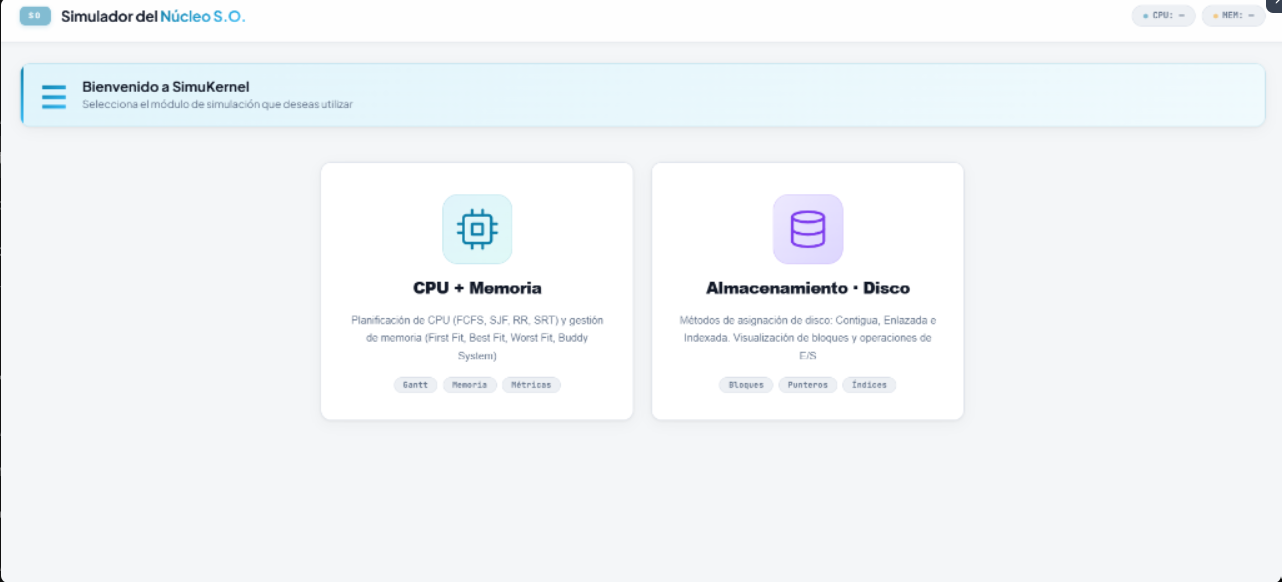
\includegraphics[width=0.9\textwidth]{imagenes/home.png}
\end{figure}

La Figura 1 muestra la pantalla de bienvenida del sistema. Desde ahí se puede acceder directamente a la interfaz de gestión de almacenamiento en disco.

\begin{figure}[H]
    \caption{\textit{Panel de configuración: selección del método y ajuste de parámetros físicos del disco}}
    \centering
    \vspace{0.3cm}
    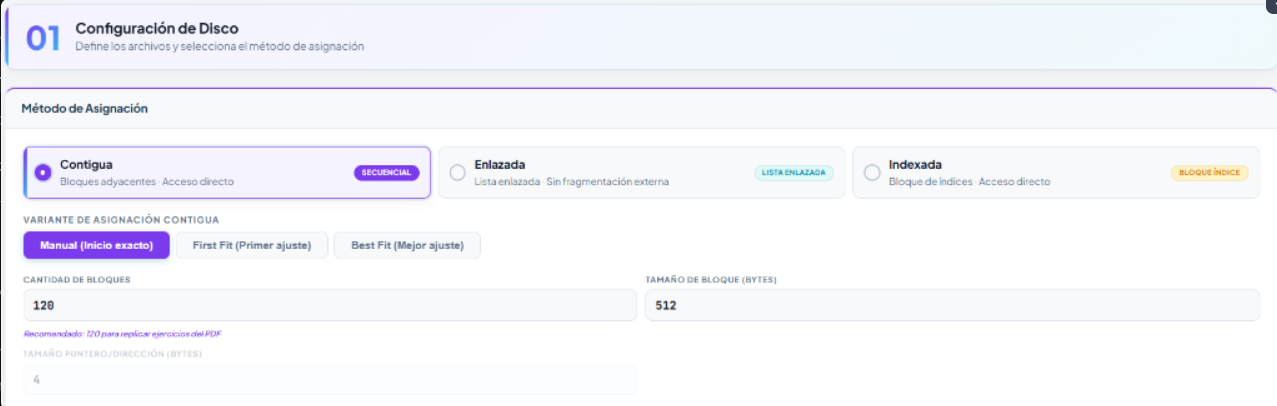
\includegraphics[width=0.9\textwidth]{imagenes/parametros.png}
\end{figure}

En la Figura 2 vemos la sección de configuración. Lo interesante aquí es que el usuario no solo elige el método, sino que también puede afinar los detalles físicos: para la asignación Contigua puede seleccionar si quiere definir el bloque de inicio a mano o dejar que el simulador lo calcule con First Fit o Best Fit. Más abajo se configuran la cantidad de bloques del disco (recomendamos 120 para que coincida con los ejercicios del material del curso), el tamaño de cada bloque en bytes y el tamaño del puntero, este último es clave porque el simulador lo usa para calcular cuánto espacio real le queda a cada bloque para datos de usuario en la asignación enlazada.

\begin{figure}[H]
    \caption{\textit{Zona de carga de archivos: importación CSV o edición manual adaptativa}}
    \centering
    \vspace{0.3cm}
    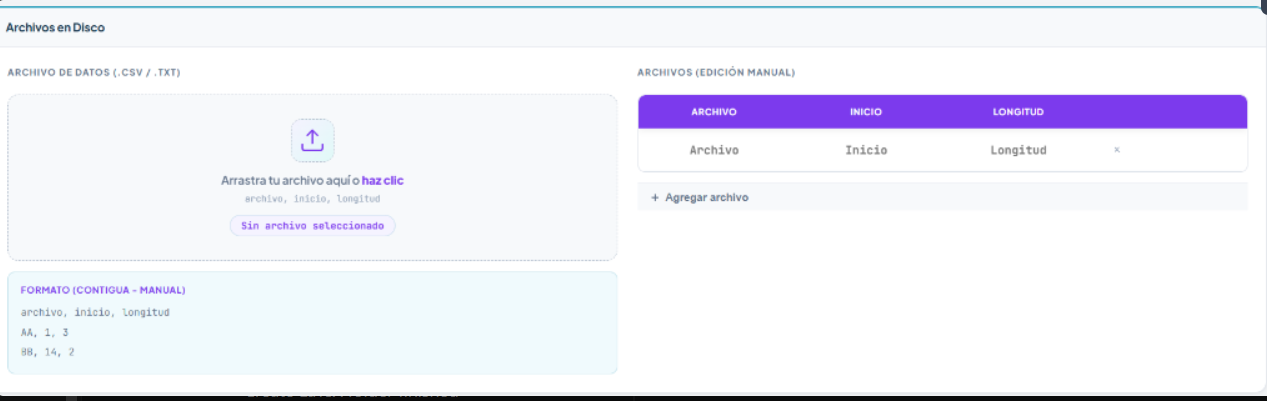
\includegraphics[width=0.9\textwidth]{imagenes/archivos.png}
\end{figure}

La Figura 3 muestra las dos formas de ingresar los datos al simulador. La más rápida es arrastrar un archivo \texttt{.csv} o \texttt{.txt} directamente a la zona de carga; el simulador lo lee automáticamente y llena la tabla. La otra opción es escribirlo a mano fila por fila, y lo que nos pareció muy práctico es que las columnas de la tabla cambian solas según el método que hayas elegido, por lo que no hay que adivinar qué datos ingresar.

\begin{figure}[H]
    \caption{\textit{Panel de simulación mostrando métricas calculadas en tiempo real}}
    \centering
    \vspace{0.3cm}
    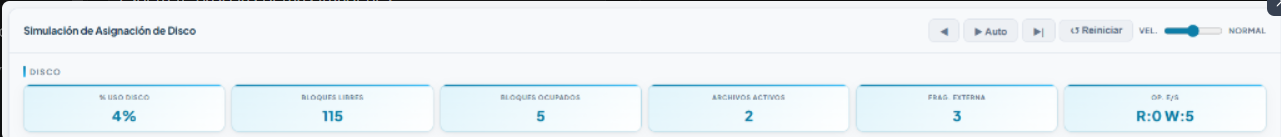
\includegraphics[width=0.9\textwidth]{imagenes/metricas.png}
\end{figure}

En la Figura 4 se puede ver el panel de control durante la ejecución. Arriba están los botones del reproductor (retroceder, reproducir automáticamente, avanzar paso a paso y reiniciar) y el slider de velocidad, que tiene cinco niveles desde muy lento hasta máximo. Debajo aparece el panel de métricas que se actualiza en tiempo real conforme avanza cada paso de la simulación, mostrando desde el porcentaje de uso del disco hasta las operaciones de escritura acumuladas.

A continuación, se presentan los resultados de las tres simulaciones realizadas con los datos de prueba del material teórico del curso.

Para generar la simulación del método contiguo, se utilizaron los siguientes datos de entrada:

\begin{table}[H]
    \centering
    \caption{\textit{Datos de Entrada para la Simulación de Asignación Contigua}}
    \vspace{0.3cm}
    \begin{tabular}{lcc}
        \toprule
        \textbf{Archivo} & \textbf{Inicio} & \textbf{Longitud (bloques)} \\
        \midrule
        AA & 1 & 3 \\
        BB & 14 & 2 \\
        \bottomrule
    \end{tabular}
\end{table}

\begin{figure}[H]
    \caption{\textit{Mapa de bloques para el método contiguo: asignación secuencial de AA y BB}}
    \centering
    \vspace{0.3cm}
    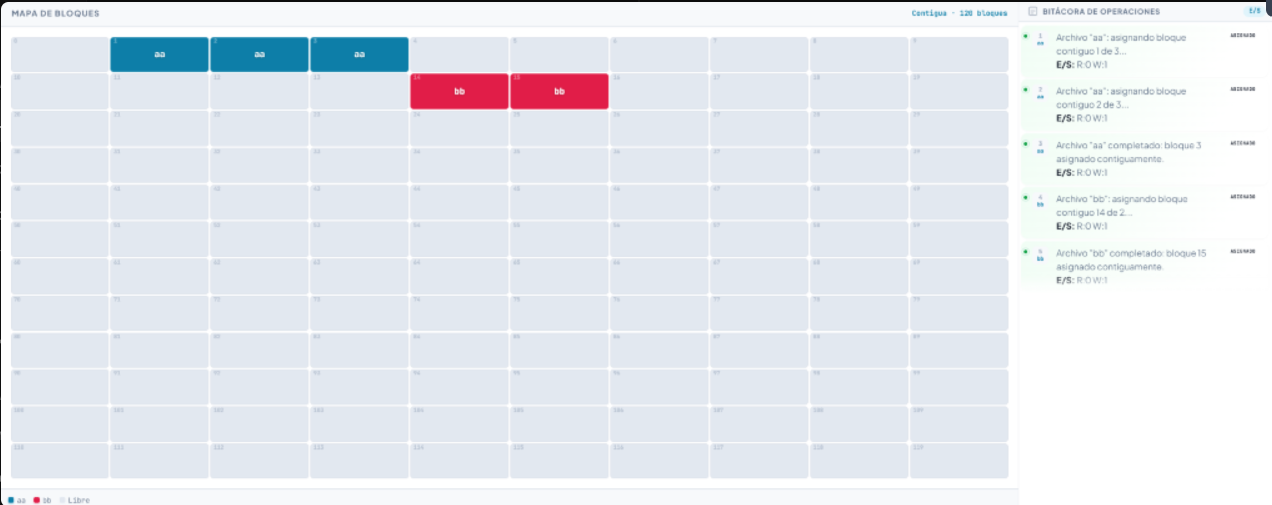
\includegraphics[width=1\textwidth]{imagenes/mapa_contigua.png}
\end{figure}

La Figura 5 muestra el resultado de la asignación contigua. Se nota claramente que \texttt{AA} quedó en los bloques 1, 2 y 3 (en azul) y \texttt{BB} en los bloques 14 y 15 (en rojo), con un hueco de 10 bloques vacíos en el medio. La bitácora de la derecha registró las 5 escrituras individuales que el simulador fue ejecutando una por una. Lo interesante es que aunque visualmente haya espacio, si intentáramos guardar un archivo de 11 bloques el sistema lo rechazaría porque no hay 11 bloques contiguos disponibles, y ese es exactamente el problema de la fragmentación externa que tanto discutimos en la teoría.

Para la prueba de la asignación enlazada, los datos ingresados fueron los siguientes:

\begin{table}[H]
    \centering
    \caption{\textit{Datos de Entrada para la Simulación de Asignación Enlazada}}
    \vspace{0.3cm}
    \begin{tabular}{ll}
        \toprule
        \textbf{Archivo} & \textbf{Secuencia de Bloques} \\
        \midrule
        AA & 6, 14, 26, 119, 8 \\
        \bottomrule
    \end{tabular}
\end{table}

\begin{figure}[H]
    \caption{\textit{Mapa de bloques enlazado: archivo AA disperso con punteros visibles en cada celda}}
    \centering
    \vspace{0.3cm}
    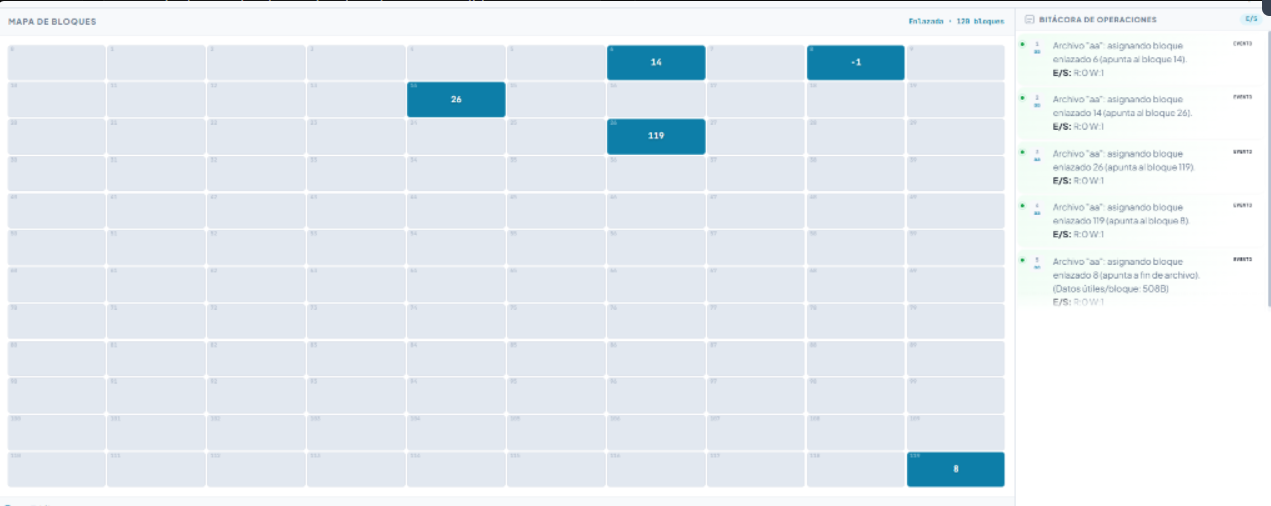
\includegraphics[width=1\textwidth]{imagenes/mapa_enlazada.png}
\end{figure}

La Figura 6 es quizás la más llamativa visualmente. Se puede ver el archivo \texttt{AA} completamente disperso por el disco, saltando del bloque 6 al 14, luego al 26, después al 119 y finalmente al 8. Dentro de cada celda aparece el número del bloque siguiente, que es el puntero. El último bloque, el 8, muestra el valor \texttt{-1} que indica que ahí termina el archivo. El simulador también nos mostró un dato concreto: con bloques de 512 B y punteros de 4 B, cada bloque solo puede guardar 508 B de datos reales, los otros 4 B se los come el puntero.

Finalmente, para la demostración de la asignación indexada, la configuración suministrada fue:

\begin{table}[H]
    \centering
    \caption{\textit{Datos de Entrada para la Simulación de Asignación Indexada}}
    \vspace{0.3cm}
    \begin{tabular}{lll}
        \toprule
        \textbf{Archivo} & \textbf{Bloque Índice} & \textbf{Bloques de Datos} \\
        \midrule
        AA & 10 & 1, 7, 3 \\
        \bottomrule
    \end{tabular}
\end{table}

\begin{figure}[H]
    \caption{\textit{Mapa de bloques indexado: bloque índice 10 referenciando los datos de AA}}
    \centering
    \vspace{0.3cm}
    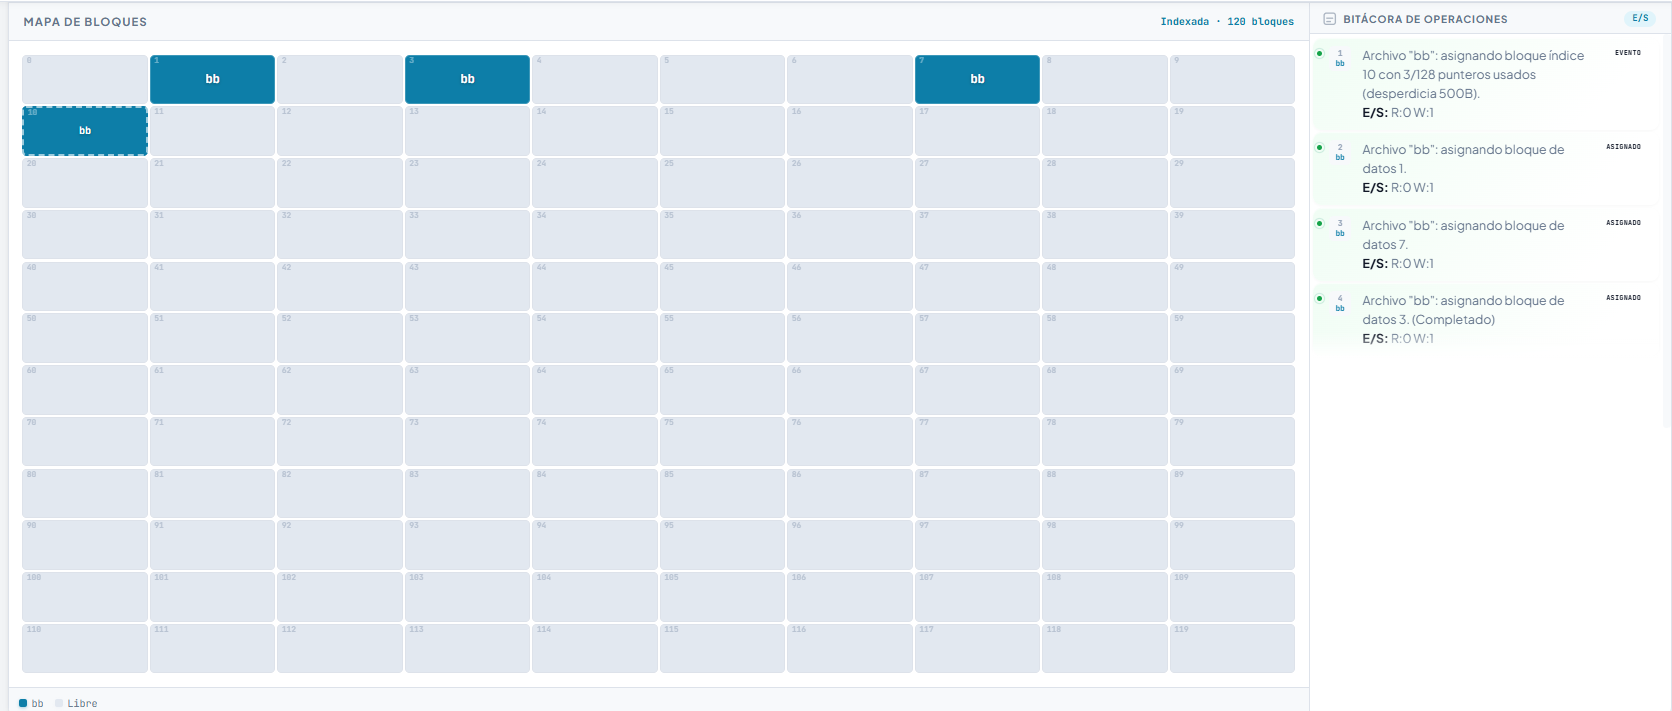
\includegraphics[width=1\textwidth]{imagenes/mapa_indexada.png}
\end{figure}

La Figura 7 muestra la asignación indexada. El bloque 10 aparece diferenciado visualmente como el bloque índice y desde él se apunta a los bloques de datos 1, 7 y 3. Lo que más llama la atención al revisar la bitácora es el primer mensaje que generó el simulador: el bloque índice solo usó 3 de los 128 punteros que podría tener, desperdiciando 500 de sus 512 bytes. Este dato, que aparece en pantalla, evidencia de manera muy gráfica el costo estructural que tiene este método cuando los archivos son pequeños.

% ---------------------------------------------------------
% 6. CONCLUSIONES
% ---------------------------------------------------------
\newpage
\section{Conclusiones}

Desarrollar este simulador resultó ser una de las prácticas más enriquecedoras del curso, porque obligó a entender los algoritmos a fondo, no solo a memorizarlos. Al observar el disco animarse bloque por bloque en la pantalla, quedó muy claro algo que la teoría menciona pero que cuesta dimensionar: ningún método es perfecto. La asignación contigua es la más rápida y simple, pero basta con simular dos archivos para ver cómo empieza a aparecer ese hueco inutilizable en el medio del disco, validando empíricamente la fragmentación externa.

Con la asignación enlazada se comprendió que solucionar la fragmentación tiene un precio. Esos 4 bytes que se le restan a cada bloque para guardar el puntero parecen poca cosa, pero el simulador dejó en evidencia que en un disco real con millones de bloques ese ``impuesto'' se acumula de forma significativa. Además, la forma en que los bloques quedan dispersos por toda la grilla hace muy visual por qué el acceso directo al centro del archivo se vuelve lento.

La asignación indexada fue quizás la más sorprendente, sobre todo cuando el simulador reportó que el bloque índice del archivo \texttt{AA} desperdiciaba 500 de sus 512 bytes para guardar apenas tres punteros. Ese dato concreto, apareciendo en tiempo real en la bitácora mientras corría la simulación, resulta pedagógicamente más potente que cualquier párrafo de un libro de texto.

En resumen, SimuKernel cumplió con creces el objetivo planteado: convertir conceptos que suelen quedarse en lo abstracto en algo que se puede ver, controlar y medir. El hecho de que todo haya sido construido con tecnologías web puras demuestra además que no se necesitan herramientas complejas para desarrollar algo con valor didáctico real.

% ---------------------------------------------------------
% 7. REFERENCIAS
% ---------------------------------------------------------
\newpage
\section{Referencias}
\vspace{-0.5cm}
\setlength{\parindent}{0cm}

\noindent
\hangindent=1.27cm
Silberschatz, A., Galvin, P. B., \& Gagne, G. (2018). \textit{Operating system concepts} (10ma ed.). Wiley.

\vspace{0.3cm}
\noindent
\hangindent=1.27cm
Stallings, W. (2018). \textit{Operating Systems: Internals and Design Principles} (9na ed.). Pearson.

\vspace{0.3cm}
\noindent
\hangindent=1.27cm
Tanenbaum, A. S., \& Bos, H. (2015). \textit{Modern operating systems} (4ta ed.). Pearson.

% ---------------------------------------------------------
% 8. ANEXOS
% ---------------------------------------------------------
\vspace{1cm}
\setlength{\parindent}{1.27cm}
\section{Anexos}

\subsection{Anexo A: Repositorio del Proyecto}

El código fuente completo del simulador SimuKernel se encuentra disponible de forma pública en el siguiente repositorio de GitHub:

\begin{center}
    \url{https://github.com/Abad-cyber/Sistema-del-nucleo-S.O..git}
\end{center}

El repositorio incluye todos los componentes del proyecto: los algoritmos de simulación, el motor de renderizado visual, los estilos CSS y la interfaz HTML principal, listos para ejecutarse localmente con cualquier servidor web estático.

\subsection{Anexo B: Manual de Usuario (Resumen)}

El uso del simulador de disco sigue tres pasos básicos:

\begin{enumerate}
    \item \textbf{Ingresar a la simulación:} Desde la pantalla de inicio, hacer clic en la tarjeta \textit{Almacenamiento · Disco}.
    \item \textbf{Configurar los parámetros:} En la sección de parámetros, elegir el método de asignación (Contigua, Enlazada o Indexada), la variante si corresponde (Manual, First Fit o Best Fit), la cantidad de bloques del disco y el tamaño de bloque en bytes.
    \item \textbf{Ingresar los archivos:} Escribir los datos directamente en la tabla de edición o cargar un archivo \texttt{.csv} o \texttt{.txt} arrastrándolo a la zona de carga. El formato varía por método:
    \begin{itemize}
        \item Contigua manual: \texttt{nombre, inicio, longitud}
        \item Enlazada: \texttt{nombre, bloque1, bloque2, \ldots}
        \item Indexada: \texttt{nombre, bloque\_indice, dato1, dato2, \ldots}
    \end{itemize}
    \item \textbf{Ejecutar la simulación:} Pulsar el botón \textit{Simular Disco}. La animación avanzará bloque por bloque de forma automática. Se puede pausar, retroceder, avanzar manualmente o ajustar la velocidad con el control deslizante (cinco niveles: Muy lento a Máximo).
\end{enumerate}

\end{document}
